\documentclass[1p]{elsarticle_modified}
%\bibliographystyle{elsarticle-num}

%\usepackage[colorlinks]{hyperref}
%\usepackage{abbrmath_seonhwa} %\Abb, \Ascr, \Acal ,\Abf, \Afrak
\usepackage{amsfonts}
\usepackage{amssymb}
\usepackage{amsmath}
\usepackage{amsthm}
\usepackage{scalefnt}
\usepackage{amsbsy}
\usepackage{kotex}
\usepackage{caption}
\usepackage{subfig}
\usepackage{color}
\usepackage{graphicx}
\usepackage{xcolor} %% white, black, red, green, blue, cyan, magenta, yellow
\usepackage{float}
\usepackage{setspace}
\usepackage{hyperref}

\usepackage{tikz}
\usetikzlibrary{arrows}

\usepackage{multirow}
\usepackage{array} % fixed length table
\usepackage{hhline}

%%%%%%%%%%%%%%%%%%%%%
\makeatletter
\renewcommand*\env@matrix[1][\arraystretch]{%
	\edef\arraystretch{#1}%
	\hskip -\arraycolsep
	\let\@ifnextchar\new@ifnextchar
	\array{*\c@MaxMatrixCols c}}
\makeatother %https://tex.stackexchange.com/questions/14071/how-can-i-increase-the-line-spacing-in-a-matrix
%%%%%%%%%%%%%%%

\usepackage[normalem]{ulem}

\newcommand{\msout}[1]{\ifmmode\text{\sout{\ensuremath{#1}}}\else\sout{#1}\fi}
%SOURCE: \msout is \stkout macro in https://tex.stackexchange.com/questions/20609/strikeout-in-math-mode

\newcommand{\cancel}[1]{
	\ifmmode
	{\color{red}\msout{#1}}
	\else
	{\color{red}\sout{#1}}
	\fi
}

\newcommand{\add}[1]{
	{\color{blue}\uwave{#1}}
}

\newcommand{\replace}[2]{
	\ifmmode
	{\color{red}\msout{#1}}{\color{blue}\uwave{#2}}
	\else
	{\color{red}\sout{#1}}{\color{blue}\uwave{#2}}
	\fi
}

\newcommand{\Sol}{\mathcal{S}} %segment
\newcommand{\D}{D} %diagram
\newcommand{\A}{\mathcal{A}} %arc


%%%%%%%%%%%%%%%%%%%%%%%%%%%%%5 test

\def\sl{\operatorname{\textup{SL}}(2,\Cbb)}
\def\psl{\operatorname{\textup{PSL}}(2,\Cbb)}
\def\quan{\mkern 1mu \triangleright \mkern 1mu}

\theoremstyle{definition}
\newtheorem{thm}{Theorem}[section]
\newtheorem{prop}[thm]{Proposition}
\newtheorem{lem}[thm]{Lemma}
\newtheorem{ques}[thm]{Question}
\newtheorem{cor}[thm]{Corollary}
\newtheorem{defn}[thm]{Definition}
\newtheorem{exam}[thm]{Example}
\newtheorem{rmk}[thm]{Remark}
\newtheorem{alg}[thm]{Algorithm}

\newcommand{\I}{\sqrt{-1}}
\begin{document}

%\begin{frontmatter}
%
%\title{Boundary parabolic representations of knots up to 8 crossings}
%
%%% Group authors per affiliation:
%\author{Yunhi Cho} 
%\address{Department of Mathematics, University of Seoul, Seoul, Korea}
%\ead{yhcho@uos.ac.kr}
%
%
%\author{Seonhwa Kim} %\fnref{s_kim}}
%\address{Center for Geometry and Physics, Institute for Basic Science, Pohang, 37673, Korea}
%\ead{ryeona17@ibs.re.kr}
%
%\author{Hyuk Kim}
%\address{Department of Mathematical Sciences, Seoul National University, Seoul 08826, Korea}
%\ead{hyukkim@snu.ac.kr}
%
%\author{Seokbeom Yoon}
%\address{Department of Mathematical Sciences, Seoul National University, Seoul, 08826,  Korea}
%\ead{sbyoon15@snu.ac.kr}
%
%\begin{abstract}
%We find all boundary parabolic representation of knots up to 8 crossings.
%
%\end{abstract}
%\begin{keyword}
%    \MSC[2010] 57M25 
%\end{keyword}
%
%\end{frontmatter}

%\linenumbers
%\tableofcontents
%
\newcommand\colored[1]{\textcolor{white}{\rule[-0.35ex]{0.8em}{1.4ex}}\kern-0.8em\color{red} #1}%
%\newcommand\colored[1]{\textcolor{white}{ #1}\kern-2.17ex	\textcolor{white}{ #1}\kern-1.81ex	\textcolor{white}{ #1}\kern-2.15ex\color{red}#1	}

{\Large $\underline{12a_{0810}~(K12a_{0810})}$}

\setlength{\tabcolsep}{10pt}
\renewcommand{\arraystretch}{1.6}
\vspace{1cm}\begin{tabular}{m{100pt}>{\centering\arraybackslash}m{274pt}}
\multirow{5}{120pt}{
	\centering
	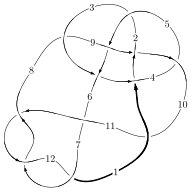
\includegraphics[width=112pt]{../../../GIT/diagram.site/Diagrams/png/1611_12a_0810.png}\\
\ \ \ A knot diagram\footnotemark}&
\allowdisplaybreaks
\textbf{Linearized knot diagam} \\
\cline{2-2}
 &
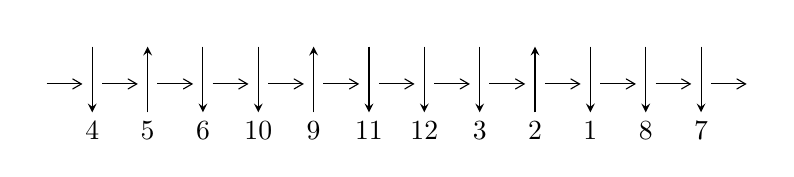
\begin{tikzpicture}[x=20pt, y=17pt]
	% nodes
	\node (C0) at (0, 0) {};
	\node (C1) at (1, 0) {};
	\node (C1U) at (1, +1) {};
	\node (C1D) at (1, -1) {4};

	\node (C2) at (2, 0) {};
	\node (C2U) at (2, +1) {};
	\node (C2D) at (2, -1) {5};

	\node (C3) at (3, 0) {};
	\node (C3U) at (3, +1) {};
	\node (C3D) at (3, -1) {6};

	\node (C4) at (4, 0) {};
	\node (C4U) at (4, +1) {};
	\node (C4D) at (4, -1) {10};

	\node (C5) at (5, 0) {};
	\node (C5U) at (5, +1) {};
	\node (C5D) at (5, -1) {9};

	\node (C6) at (6, 0) {};
	\node (C6U) at (6, +1) {};
	\node (C6D) at (6, -1) {11};

	\node (C7) at (7, 0) {};
	\node (C7U) at (7, +1) {};
	\node (C7D) at (7, -1) {12};

	\node (C8) at (8, 0) {};
	\node (C8U) at (8, +1) {};
	\node (C8D) at (8, -1) {3};

	\node (C9) at (9, 0) {};
	\node (C9U) at (9, +1) {};
	\node (C9D) at (9, -1) {2};

	\node (C10) at (10, 0) {};
	\node (C10U) at (10, +1) {};
	\node (C10D) at (10, -1) {1};

	\node (C11) at (11, 0) {};
	\node (C11U) at (11, +1) {};
	\node (C11D) at (11, -1) {8};

	\node (C12) at (12, 0) {};
	\node (C12U) at (12, +1) {};
	\node (C12D) at (12, -1) {7};
	\node (C13) at (13, 0) {};

	% arrows
	\draw[->,>={angle 60}]
	(C0) edge (C1) (C1) edge (C2) (C2) edge (C3) (C3) edge (C4) (C4) edge (C5) (C5) edge (C6) (C6) edge (C7) (C7) edge (C8) (C8) edge (C9) (C9) edge (C10) (C10) edge (C11) (C11) edge (C12) (C12) edge (C13) ;	\draw[->,>=stealth]
	(C1U) edge (C1D) (C2D) edge (C2U) (C3U) edge (C3D) (C4U) edge (C4D) (C5D) edge (C5U) (C6U) edge (C6D) (C7U) edge (C7D) (C8U) edge (C8D) (C9D) edge (C9U) (C10U) edge (C10D) (C11U) edge (C11D) (C12U) edge (C12D) ;
	\end{tikzpicture} \\
\hhline{~~} \\& 
\textbf{Solving Sequence} \\ \cline{2-2} 
 &
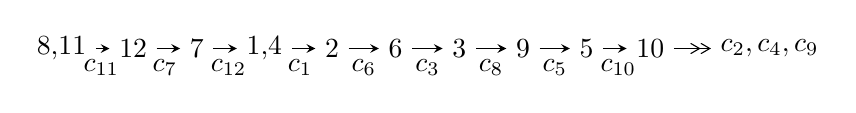
\begin{tikzpicture}[x=23pt, y=7pt]
	% node
	\node (A0) at (-1/8, 0) {8,11};
	\node (A1) at (1, 0) {12};
	\node (A2) at (2, 0) {7};
	\node (A3) at (49/16, 0) {1,4};
	\node (A4) at (33/8, 0) {2};
	\node (A5) at (41/8, 0) {6};
	\node (A6) at (49/8, 0) {3};
	\node (A7) at (57/8, 0) {9};
	\node (A8) at (65/8, 0) {5};
	\node (A9) at (73/8, 0) {10};
	\node (C1) at (1/2, -1) {$c_{11}$};
	\node (C2) at (3/2, -1) {$c_{7}$};
	\node (C3) at (5/2, -1) {$c_{12}$};
	\node (C4) at (29/8, -1) {$c_{1}$};
	\node (C5) at (37/8, -1) {$c_{6}$};
	\node (C6) at (45/8, -1) {$c_{3}$};
	\node (C7) at (53/8, -1) {$c_{8}$};
	\node (C8) at (61/8, -1) {$c_{5}$};
	\node (C9) at (69/8, -1) {$c_{10}$};
	\node (A10) at (11, 0) {$c_{2},c_{4},c_{9}$};

	% edge
	\draw[->,>=stealth]	
	(A0) edge (A1) (A1) edge (A2) (A2) edge (A3) (A3) edge (A4) (A4) edge (A5) (A5) edge (A6) (A6) edge (A7) (A7) edge (A8) (A8) edge (A9) ;
	\draw[->>,>={angle 60}]	
	(A9) edge (A10);
\end{tikzpicture} \\ 

\end{tabular} \\

\footnotetext{
The image of knot diagram is generated by the software ``\textbf{Draw programme}" developed by Andrew Bartholomew(\url{http://www.layer8.co.uk/maths/draw/index.htm\#Running-draw}), where we modified some parts for our purpose(\url{https://github.com/CATsTAILs/LinksPainter}).
}\phantom \\ \newline 
\centering \textbf{Ideals for irreducible components\footnotemark of $X_{\text{par}}$} 
 
\begin{align*}
I^u_{1}&=\langle 
-53291 u^{57}-330291 u^{56}+\cdots+14534 b-482502,\\
\phantom{I^u_{1}}&\phantom{= \langle  }-241251 u^{57}-1340924 u^{56}+\cdots+29068 a-1111355,\;u^{58}+6 u^{57}+\cdots+37 u+4\rangle \\
I^u_{2}&=\langle 
-2 u^{40}+3 u^{39}+\cdots+b+3,\;3 u^{42} a+11 u^{42}+\cdots-6 a-25,\;u^{43}-2 u^{42}+\cdots-6 u+1\rangle \\
I^u_{3}&=\langle 
- u^{15}+u^{14}-7 u^{13}+6 u^{12}-20 u^{11}+12 u^{10}-29 u^9+6 u^8-20 u^7-8 u^6-10 u^4+7 u^3-5 u^2+b+u-2,\\
\phantom{I^u_{3}}&\phantom{= \langle  }2 u^{16}-2 u^{15}+\cdots+a-3,\;u^{17}- u^{16}+\cdots-2 u+1\rangle \\
I^u_{4}&=\langle 
a u- u^2+b- u-1,\;u^2 a+a^2+2 u^2+a+u+3,\;u^3+u^2+2 u+1\rangle \\
\\
\end{align*}
\raggedright * 4 irreducible components of $\dim_{\mathbb{C}}=0$, with total 167 representations.\\
\footnotetext{All coefficients of polynomials are rational numbers. But the coefficients are sometimes approximated in decimal forms when there is not enough margin.}
\newpage
\renewcommand{\arraystretch}{1}
\centering \section*{I. $I^u_{1}= \langle -5.33\times10^{4} u^{57}-3.30\times10^{5} u^{56}+\cdots+1.45\times10^{4} b-4.83\times10^{5},\;-2.41\times10^{5} u^{57}-1.34\times10^{6} u^{56}+\cdots+2.91\times10^{4} a-1.11\times10^{6},\;u^{58}+6 u^{57}+\cdots+37 u+4 \rangle$}
\flushleft \textbf{(i) Arc colorings}\\
\begin{tabular}{m{7pt} m{180pt} m{7pt} m{180pt} }
\flushright $a_{8}=$&$\begin{pmatrix}0\\u\end{pmatrix}$ \\
\flushright $a_{11}=$&$\begin{pmatrix}1\\0\end{pmatrix}$ \\
\flushright $a_{12}=$&$\begin{pmatrix}1\\u^2\end{pmatrix}$ \\
\flushright $a_{7}=$&$\begin{pmatrix}u\\u^3+u\end{pmatrix}$ \\
\flushright $a_{1}=$&$\begin{pmatrix}u^2+1\\u^4+2 u^2\end{pmatrix}$ \\
\flushright $a_{4}=$&$\begin{pmatrix}8.29954 u^{57}+46.1306 u^{56}+\cdots+337.485 u+38.2329\\3.66664 u^{57}+22.7254 u^{56}+\cdots+268.850 u+33.1982\end{pmatrix}$ \\
\flushright $a_{2}=$&$\begin{pmatrix}-2.89765 u^{57}-15.3587 u^{56}+\cdots-105.156 u-12.0214\\-2.02725 u^{57}-12.7218 u^{56}+\cdots-94.1918 u-11.5906\end{pmatrix}$ \\
\flushright $a_{6}=$&$\begin{pmatrix}u^3+2 u\\u^3+u\end{pmatrix}$ \\
\flushright $a_{3}=$&$\begin{pmatrix}3.21223 u^{57}+16.7379 u^{56}+\cdots+84.4613 u+8.61301\\2.41510 u^{57}+14.4401 u^{56}+\cdots+114.725 u+14.5737\end{pmatrix}$ \\
\flushright $a_{9}=$&$\begin{pmatrix}-2.60875 u^{57}-12.7540 u^{56}+\cdots-168.192 u-25.1931\\-4.24625 u^{57}-24.3533 u^{56}+\cdots-130.976 u-17.3985\end{pmatrix}$ \\
\flushright $a_{5}=$&$\begin{pmatrix}7.39765 u^{57}+42.3587 u^{56}+\cdots+357.156 u+41.5214\\1.63940 u^{57}+11.0036 u^{56}+\cdots+286.658 u+36.6075\end{pmatrix}$ \\
\flushright $a_{10}=$&$\begin{pmatrix}- u^6-3 u^4-2 u^2+1\\- u^8-4 u^6-4 u^4\end{pmatrix}$\\&\end{tabular}
\flushleft \textbf{(ii) Obstruction class $= -1$}\\~\\
\flushleft \textbf{(iii) Cusp Shapes $= -\frac{47209}{7267} u^{57}-\frac{39509}{1118} u^{56}+\cdots-\frac{5750393}{14534} u-\frac{461504}{7267}$}\\~\\
\newpage\renewcommand{\arraystretch}{1}
\flushleft \textbf{(iv) u-Polynomials at the component}\newline \\
\begin{tabular}{m{50pt}|m{274pt}}
Crossings & \hspace{64pt}u-Polynomials at each crossing \\
\hline $$\begin{aligned}c_{1},c_{3}\end{aligned}$$&$\begin{aligned}
&u^{58}+10 u^{57}+\cdots-5 u+1
\end{aligned}$\\
\hline $$\begin{aligned}c_{2}\end{aligned}$$&$\begin{aligned}
&u^{58}+30 u^{57}+\cdots+7 u+2
\end{aligned}$\\
\hline $$\begin{aligned}c_{4},c_{8}\end{aligned}$$&$\begin{aligned}
&u^{58}+8 u^{56}+\cdots+5 u+2
\end{aligned}$\\
\hline $$\begin{aligned}c_{5},c_{9}\end{aligned}$$&$\begin{aligned}
&u^{58}-2 u^{57}+\cdots- u+1
\end{aligned}$\\
\hline $$\begin{aligned}c_{6}\end{aligned}$$&$\begin{aligned}
&u^{58}-6 u^{57}+\cdots+10406 u+1768
\end{aligned}$\\
\hline $$\begin{aligned}c_{7},c_{11},c_{12}\end{aligned}$$&$\begin{aligned}
&u^{58}+6 u^{57}+\cdots+37 u+4
\end{aligned}$\\
\hline $$\begin{aligned}c_{10}\end{aligned}$$&$\begin{aligned}
&u^{58}-10 u^{57}+\cdots-79407 u+9248
\end{aligned}$\\
\hline
\end{tabular}\\~\\
\newpage\renewcommand{\arraystretch}{1}
\flushleft \textbf{(v) Riley Polynomials at the component}\newline \\
\begin{tabular}{m{50pt}|m{274pt}}
Crossings & \hspace{64pt}Riley Polynomials at each crossing \\
\hline $$\begin{aligned}c_{1},c_{3}\end{aligned}$$&$\begin{aligned}
&y^{58}-20 y^{57}+\cdots-37 y+1
\end{aligned}$\\
\hline $$\begin{aligned}c_{2}\end{aligned}$$&$\begin{aligned}
&y^{58}+12 y^{56}+\cdots-17 y+4
\end{aligned}$\\
\hline $$\begin{aligned}c_{4},c_{8}\end{aligned}$$&$\begin{aligned}
&y^{58}+16 y^{57}+\cdots+47 y+4
\end{aligned}$\\
\hline $$\begin{aligned}c_{5},c_{9}\end{aligned}$$&$\begin{aligned}
&y^{58}+32 y^{57}+\cdots+67 y+1
\end{aligned}$\\
\hline $$\begin{aligned}c_{6}\end{aligned}$$&$\begin{aligned}
&y^{58}+14 y^{57}+\cdots+31546284 y+3125824
\end{aligned}$\\
\hline $$\begin{aligned}c_{7},c_{11},c_{12}\end{aligned}$$&$\begin{aligned}
&y^{58}+54 y^{57}+\cdots-89 y+16
\end{aligned}$\\
\hline $$\begin{aligned}c_{10}\end{aligned}$$&$\begin{aligned}
&y^{58}+30 y^{57}+\cdots+1679029599 y+85525504
\end{aligned}$\\
\hline
\end{tabular}\\~\\
\newpage\flushleft \textbf{(vi) Complex Volumes and Cusp Shapes}
$$\begin{array}{c|c|c}  
\text{Solutions to }I^u_{1}& \I (\text{vol} + \sqrt{-1}CS) & \text{Cusp shape}\\
 \hline 
\begin{aligned}
u &= -0.486650 + 0.826191 I \\
a &= \phantom{-}0.344322 - 0.261471 I \\
b &= -0.048461 - 0.411721 I\end{aligned}
 & \phantom{-}0.75504 + 4.17161 I & -17.2218 - 16.9606 I \\ \hline\begin{aligned}
u &= -0.486650 - 0.826191 I \\
a &= \phantom{-}0.344322 + 0.261471 I \\
b &= -0.048461 + 0.411721 I\end{aligned}
 & \phantom{-}0.75504 - 4.17161 I & -17.2218 + 16.9606 I \\ \hline\begin{aligned}
u &= \phantom{-}0.305000 + 1.120370 I \\
a &= \phantom{-}0.337905 - 0.211727 I \\
b &= -0.340274 - 0.314004 I\end{aligned}
 & -0.40781 + 4.56651 I & \phantom{-0.000000 } 0 \\ \hline\begin{aligned}
u &= \phantom{-}0.305000 - 1.120370 I \\
a &= \phantom{-}0.337905 + 0.211727 I \\
b &= -0.340274 + 0.314004 I\end{aligned}
 & -0.40781 - 4.56651 I & \phantom{-0.000000 } 0 \\ \hline\begin{aligned}
u &= -0.683075 + 0.462128 I \\
a &= -0.542422 + 1.104780 I \\
b &= \phantom{-}0.140036 + 1.005320 I\end{aligned}
 & \phantom{-}0.22278 + 2.22232 I & -13.09381 - 5.11160 I \\ \hline\begin{aligned}
u &= -0.683075 - 0.462128 I \\
a &= -0.542422 - 1.104780 I \\
b &= \phantom{-}0.140036 - 1.005320 I\end{aligned}
 & \phantom{-}0.22278 - 2.22232 I & -13.09381 + 5.11160 I \\ \hline\begin{aligned}
u &= -0.537460 + 0.617600 I \\
a &= \phantom{-}1.94977 + 0.77515 I \\
b &= \phantom{-}1.52666 - 0.78757 I\end{aligned}
 & \phantom{-}2.39350 - 11.33360 I & -3.90914 + 5.14948 I \\ \hline\begin{aligned}
u &= -0.537460 - 0.617600 I \\
a &= \phantom{-}1.94977 - 0.77515 I \\
b &= \phantom{-}1.52666 + 0.78757 I\end{aligned}
 & \phantom{-}2.39350 + 11.33360 I & -3.90914 - 5.14948 I \\ \hline\begin{aligned}
u &= -0.729161 + 0.366582 I \\
a &= -1.28232 - 2.43009 I \\
b &= -1.82584 - 1.30185 I\end{aligned}
 & \phantom{-}1.4886 + 15.6557 I & -5.70789 - 10.38760 I \\ \hline\begin{aligned}
u &= -0.729161 - 0.366582 I \\
a &= -1.28232 + 2.43009 I \\
b &= -1.82584 + 1.30185 I\end{aligned}
 & \phantom{-}1.4886 - 15.6557 I & -5.70789 + 10.38760 I\\
 \hline 
 \end{array}$$\newpage$$\begin{array}{c|c|c}  
\text{Solutions to }I^u_{1}& \I (\text{vol} + \sqrt{-1}CS) & \text{Cusp shape}\\
 \hline 
\begin{aligned}
u &= -0.013312 + 1.213490 I \\
a &= -1.198630 + 0.354187 I \\
b &= \phantom{-}0.41384 + 1.45923 I\end{aligned}
 & \phantom{-}0.694497 + 0.076769 I & \phantom{-0.000000 } 0 \\ \hline\begin{aligned}
u &= -0.013312 - 1.213490 I \\
a &= -1.198630 - 0.354187 I \\
b &= \phantom{-}0.41384 - 1.45923 I\end{aligned}
 & \phantom{-}0.694497 - 0.076769 I & \phantom{-0.000000 } 0 \\ \hline\begin{aligned}
u &= \phantom{-}0.188583 + 1.225570 I \\
a &= -0.795866 - 0.034391 I \\
b &= \phantom{-}0.107938 + 0.981875 I\end{aligned}
 & -0.66118 - 4.66603 I & \phantom{-0.000000 } 0 \\ \hline\begin{aligned}
u &= \phantom{-}0.188583 - 1.225570 I \\
a &= -0.795866 + 0.034391 I \\
b &= \phantom{-}0.107938 - 0.981875 I\end{aligned}
 & -0.66118 + 4.66603 I & \phantom{-0.000000 } 0 \\ \hline\begin{aligned}
u &= -0.667450 + 0.362079 I \\
a &= \phantom{-}1.42453 + 2.98943 I \\
b &= \phantom{-}2.03321 + 1.47950 I\end{aligned}
 & -0.49660 + 6.79598 I & -12.1715 - 9.4069 I \\ \hline\begin{aligned}
u &= -0.667450 - 0.362079 I \\
a &= \phantom{-}1.42453 - 2.98943 I \\
b &= \phantom{-}2.03321 - 1.47950 I\end{aligned}
 & -0.49660 - 6.79598 I & -12.1715 + 9.4069 I \\ \hline\begin{aligned}
u &= \phantom{-}0.748570 + 0.048874 I \\
a &= -0.400924 - 0.165680 I \\
b &= \phantom{-}0.292022 + 0.143618 I\end{aligned}
 & -3.68988 - 8.42336 I & -10.53471 + 7.87489 I \\ \hline\begin{aligned}
u &= \phantom{-}0.748570 - 0.048874 I \\
a &= -0.400924 + 0.165680 I \\
b &= \phantom{-}0.292022 - 0.143618 I\end{aligned}
 & -3.68988 + 8.42336 I & -10.53471 - 7.87489 I \\ \hline\begin{aligned}
u &= \phantom{-}0.182516 + 1.252480 I \\
a &= -0.460878 + 0.482200 I \\
b &= \phantom{-}0.688062 + 0.489231 I\end{aligned}
 & -0.537435 - 1.220210 I & \phantom{-0.000000 } 0 \\ \hline\begin{aligned}
u &= \phantom{-}0.182516 - 1.252480 I \\
a &= -0.460878 - 0.482200 I \\
b &= \phantom{-}0.688062 - 0.489231 I\end{aligned}
 & -0.537435 + 1.220210 I & \phantom{-0.000000 } 0\\
 \hline 
 \end{array}$$\newpage$$\begin{array}{c|c|c}  
\text{Solutions to }I^u_{1}& \I (\text{vol} + \sqrt{-1}CS) & \text{Cusp shape}\\
 \hline 
\begin{aligned}
u &= -0.716893 + 0.148103 I \\
a &= -0.586320 - 0.467569 I \\
b &= -0.489577 - 0.248361 I\end{aligned}
 & -1.46760 + 0.14646 I & -10.66155 - 6.45496 I \\ \hline\begin{aligned}
u &= -0.716893 - 0.148103 I \\
a &= -0.586320 + 0.467569 I \\
b &= -0.489577 + 0.248361 I\end{aligned}
 & -1.46760 - 0.14646 I & -10.66155 + 6.45496 I \\ \hline\begin{aligned}
u &= \phantom{-}0.598802 + 0.420280 I \\
a &= -0.056377 + 0.342481 I \\
b &= \phantom{-}0.177697 - 0.181384 I\end{aligned}
 & \phantom{-}3.17991 - 1.93750 I & -0.05128 + 3.41899 I \\ \hline\begin{aligned}
u &= \phantom{-}0.598802 - 0.420280 I \\
a &= -0.056377 - 0.342481 I \\
b &= \phantom{-}0.177697 + 0.181384 I\end{aligned}
 & \phantom{-}3.17991 + 1.93750 I & -0.05128 - 3.41899 I \\ \hline\begin{aligned}
u &= \phantom{-}0.296710 + 1.235000 I \\
a &= \phantom{-}0.503062 + 0.098001 I \\
b &= -0.028232 - 0.650361 I\end{aligned}
 & \phantom{-}0.26982 - 12.21040 I & \phantom{-0.000000 } 0 \\ \hline\begin{aligned}
u &= \phantom{-}0.296710 - 1.235000 I \\
a &= \phantom{-}0.503062 - 0.098001 I \\
b &= -0.028232 + 0.650361 I\end{aligned}
 & \phantom{-}0.26982 + 12.21040 I & \phantom{-0.000000 } 0 \\ \hline\begin{aligned}
u &= -0.498652 + 0.501751 I \\
a &= -2.45024 - 1.17096 I \\
b &= -1.80935 + 0.64551 I\end{aligned}
 & \phantom{-}0.14979 - 2.90525 I & -9.74237 + 2.76855 I \\ \hline\begin{aligned}
u &= -0.498652 - 0.501751 I \\
a &= -2.45024 + 1.17096 I \\
b &= -1.80935 - 0.64551 I\end{aligned}
 & \phantom{-}0.14979 + 2.90525 I & -9.74237 - 2.76855 I \\ \hline\begin{aligned}
u &= -0.068712 + 1.333800 I \\
a &= \phantom{-}0.769513 + 0.152421 I \\
b &= \phantom{-}0.256174 - 1.015900 I\end{aligned}
 & \phantom{-}3.90944 + 2.10883 I & \phantom{-0.000000 } 0 \\ \hline\begin{aligned}
u &= -0.068712 - 1.333800 I \\
a &= \phantom{-}0.769513 - 0.152421 I \\
b &= \phantom{-}0.256174 + 1.015900 I\end{aligned}
 & \phantom{-}3.90944 - 2.10883 I & \phantom{-0.000000 } 0\\
 \hline 
 \end{array}$$\newpage$$\begin{array}{c|c|c}  
\text{Solutions to }I^u_{1}& \I (\text{vol} + \sqrt{-1}CS) & \text{Cusp shape}\\
 \hline 
\begin{aligned}
u &= \phantom{-}0.554749 + 0.320999 I \\
a &= \phantom{-}0.363194 - 0.745212 I \\
b &= -0.440694 + 0.296820 I\end{aligned}
 & -1.24071 - 1.57402 I & -9.37561 + 4.19103 I \\ \hline\begin{aligned}
u &= \phantom{-}0.554749 - 0.320999 I \\
a &= \phantom{-}0.363194 + 0.745212 I \\
b &= -0.440694 - 0.296820 I\end{aligned}
 & -1.24071 + 1.57402 I & -9.37561 - 4.19103 I \\ \hline\begin{aligned}
u &= \phantom{-}0.620237 + 0.005952 I \\
a &= \phantom{-}0.684603 - 0.312047 I \\
b &= -0.426474 + 0.189468 I\end{aligned}
 & -4.34476 + 1.69097 I & -17.4074 - 4.2929 I \\ \hline\begin{aligned}
u &= \phantom{-}0.620237 - 0.005952 I \\
a &= \phantom{-}0.684603 + 0.312047 I \\
b &= -0.426474 - 0.189468 I\end{aligned}
 & -4.34476 - 1.69097 I & -17.4074 + 4.2929 I \\ \hline\begin{aligned}
u &= -0.552154 + 0.262175 I \\
a &= -0.00417 + 2.56788 I \\
b &= \phantom{-}0.67093 + 1.41896 I\end{aligned}
 & -1.55541 + 1.68524 I & -10.30877 - 5.83070 I \\ \hline\begin{aligned}
u &= -0.552154 - 0.262175 I \\
a &= -0.00417 - 2.56788 I \\
b &= \phantom{-}0.67093 - 1.41896 I\end{aligned}
 & -1.55541 - 1.68524 I & -10.30877 + 5.83070 I \\ \hline\begin{aligned}
u &= -0.247870 + 1.385030 I \\
a &= -0.001904 + 0.889063 I \\
b &= \phantom{-}1.230910 + 0.223010 I\end{aligned}
 & \phantom{-}3.45219 + 3.47788 I & \phantom{-0.000000 } 0 \\ \hline\begin{aligned}
u &= -0.247870 - 1.385030 I \\
a &= -0.001904 - 0.889063 I \\
b &= \phantom{-}1.230910 - 0.223010 I\end{aligned}
 & \phantom{-}3.45219 - 3.47788 I & \phantom{-0.000000 } 0 \\ \hline\begin{aligned}
u &= -0.21441 + 1.40281 I \\
a &= \phantom{-}0.99934 - 1.05859 I \\
b &= -1.27072 - 1.62886 I\end{aligned}
 & \phantom{-}3.77827 + 4.51742 I & \phantom{-0.000000 } 0 \\ \hline\begin{aligned}
u &= -0.21441 - 1.40281 I \\
a &= \phantom{-}0.99934 + 1.05859 I \\
b &= -1.27072 + 1.62886 I\end{aligned}
 & \phantom{-}3.77827 - 4.51742 I & \phantom{-0.000000 } 0\\
 \hline 
 \end{array}$$\newpage$$\begin{array}{c|c|c}  
\text{Solutions to }I^u_{1}& \I (\text{vol} + \sqrt{-1}CS) & \text{Cusp shape}\\
 \hline 
\begin{aligned}
u &= \phantom{-}0.21996 + 1.42291 I \\
a &= -0.231668 + 0.476881 I \\
b &= \phantom{-}0.729514 + 0.224747 I\end{aligned}
 & \phantom{-}4.35313 - 4.46243 I & \phantom{-0.000000 } 0 \\ \hline\begin{aligned}
u &= \phantom{-}0.21996 - 1.42291 I \\
a &= -0.231668 - 0.476881 I \\
b &= \phantom{-}0.729514 - 0.224747 I\end{aligned}
 & \phantom{-}4.35313 + 4.46243 I & \phantom{-0.000000 } 0 \\ \hline\begin{aligned}
u &= -0.18090 + 1.45437 I \\
a &= \phantom{-}0.24700 + 1.67631 I \\
b &= \phantom{-}2.48266 - 0.05598 I\end{aligned}
 & \phantom{-}6.36667 - 0.42955 I & \phantom{-0.000000 } 0 \\ \hline\begin{aligned}
u &= -0.18090 - 1.45437 I \\
a &= \phantom{-}0.24700 - 1.67631 I \\
b &= \phantom{-}2.48266 + 0.05598 I\end{aligned}
 & \phantom{-}6.36667 + 0.42955 I & \phantom{-0.000000 } 0 \\ \hline\begin{aligned}
u &= -0.25301 + 1.44537 I \\
a &= \phantom{-}0.91357 - 1.91598 I \\
b &= -2.53814 - 1.80521 I\end{aligned}
 & \phantom{-}5.31051 + 10.16090 I & \phantom{-0.000000 } 0 \\ \hline\begin{aligned}
u &= -0.25301 - 1.44537 I \\
a &= \phantom{-}0.91357 + 1.91598 I \\
b &= -2.53814 + 1.80521 I\end{aligned}
 & \phantom{-}5.31051 - 10.16090 I & \phantom{-0.000000 } 0 \\ \hline\begin{aligned}
u &= \phantom{-}0.22159 + 1.45553 I \\
a &= \phantom{-}0.072388 - 0.270086 I \\
b &= -0.409159 - 0.045515 I\end{aligned}
 & \phantom{-}9.20820 - 4.94870 I & \phantom{-0.000000 } 0 \\ \hline\begin{aligned}
u &= \phantom{-}0.22159 - 1.45553 I \\
a &= \phantom{-}0.072388 + 0.270086 I \\
b &= -0.409159 + 0.045515 I\end{aligned}
 & \phantom{-}9.20820 + 4.94870 I & \phantom{-0.000000 } 0 \\ \hline\begin{aligned}
u &= -0.27798 + 1.45411 I \\
a &= -0.70415 + 1.66871 I \\
b &= \phantom{-}2.23074 + 1.48777 I\end{aligned}
 & \phantom{-}7.3380 + 19.3241 I & \phantom{-0.000000 } 0 \\ \hline\begin{aligned}
u &= -0.27798 - 1.45411 I \\
a &= -0.70415 - 1.66871 I \\
b &= \phantom{-}2.23074 - 1.48777 I\end{aligned}
 & \phantom{-}7.3380 - 19.3241 I & \phantom{-0.000000 } 0\\
 \hline 
 \end{array}$$\newpage$$\begin{array}{c|c|c}  
\text{Solutions to }I^u_{1}& \I (\text{vol} + \sqrt{-1}CS) & \text{Cusp shape}\\
 \hline 
\begin{aligned}
u &= -0.14926 + 1.49263 I \\
a &= -0.200412 - 1.212690 I \\
b &= -1.84002 + 0.11814 I\end{aligned}
 & \phantom{-}9.24070 - 8.97855 I & \phantom{-0.000000 } 0 \\ \hline\begin{aligned}
u &= -0.14926 - 1.49263 I \\
a &= -0.200412 + 1.212690 I \\
b &= -1.84002 - 0.11814 I\end{aligned}
 & \phantom{-}9.24070 + 8.97855 I & \phantom{-0.000000 } 0 \\ \hline\begin{aligned}
u &= -0.25822 + 1.48249 I \\
a &= \phantom{-}0.628146 - 0.442430 I \\
b &= -0.493697 - 1.045470 I\end{aligned}
 & \phantom{-}6.49112 + 5.68833 I & \phantom{-0.000000 } 0 \\ \hline\begin{aligned}
u &= -0.25822 - 1.48249 I \\
a &= \phantom{-}0.628146 + 0.442430 I \\
b &= -0.493697 + 1.045470 I\end{aligned}
 & \phantom{-}6.49112 - 5.68833 I & \phantom{-0.000000 } 0 \\ \hline\begin{aligned}
u &= -0.11942 + 1.52627 I \\
a &= -0.327180 + 0.242381 I \\
b &= \phantom{-}0.330868 + 0.528310 I\end{aligned}
 & \phantom{-}8.42211 + 6.12728 I & \phantom{-0.000000 } 0 \\ \hline\begin{aligned}
u &= -0.11942 - 1.52627 I \\
a &= -0.327180 - 0.242381 I \\
b &= \phantom{-}0.330868 - 0.528310 I\end{aligned}
 & \phantom{-}8.42211 - 6.12728 I & \phantom{-0.000000 } 0 \\ \hline\begin{aligned}
u &= -0.282114 + 0.301857 I \\
a &= -1.86889 + 0.58508 I \\
b &= -0.350628 + 0.729197 I\end{aligned}
 & -0.937840 + 0.856649 I & -7.17209 - 5.06992 I \\ \hline\begin{aligned}
u &= -0.282114 - 0.301857 I \\
a &= -1.86889 - 0.58508 I \\
b &= -0.350628 - 0.729197 I\end{aligned}
 & -0.937840 - 0.856649 I & -7.17209 + 5.06992 I\\
 \hline 
 \end{array}$$\newpage\newpage\renewcommand{\arraystretch}{1}
\centering \section*{II. $I^u_{2}= \langle -2 u^{40}+3 u^{39}+\cdots+b+3,\;3 u^{42} a+11 u^{42}+\cdots-6 a-25,\;u^{43}-2 u^{42}+\cdots-6 u+1 \rangle$}
\flushleft \textbf{(i) Arc colorings}\\
\begin{tabular}{m{7pt} m{180pt} m{7pt} m{180pt} }
\flushright $a_{8}=$&$\begin{pmatrix}0\\u\end{pmatrix}$ \\
\flushright $a_{11}=$&$\begin{pmatrix}1\\0\end{pmatrix}$ \\
\flushright $a_{12}=$&$\begin{pmatrix}1\\u^2\end{pmatrix}$ \\
\flushright $a_{7}=$&$\begin{pmatrix}u\\u^3+u\end{pmatrix}$ \\
\flushright $a_{1}=$&$\begin{pmatrix}u^2+1\\u^4+2 u^2\end{pmatrix}$ \\
\flushright $a_{4}=$&$\begin{pmatrix}a\\2 u^{40}-3 u^{39}+\cdots+12 u-3\end{pmatrix}$ \\
\flushright $a_{2}=$&$\begin{pmatrix}u^{42} a- u^{42}+\cdots-2 a+4\\u^{42} a-3 u^{41} a+\cdots-2 a-1\end{pmatrix}$ \\
\flushright $a_{6}=$&$\begin{pmatrix}u^3+2 u\\u^3+u\end{pmatrix}$ \\
\flushright $a_{3}=$&$\begin{pmatrix}u^{42}-2 u^{41}+\cdots+a-2\\3 u^{40}-5 u^{39}+\cdots+15 u-4\end{pmatrix}$ \\
\flushright $a_{9}=$&$\begin{pmatrix}4 u^{42}-5 u^{41}+\cdots- a-9\\- u^{41} a+3 u^{42}+\cdots+17 u-4\end{pmatrix}$ \\
\flushright $a_{5}=$&$\begin{pmatrix}- u^{39}+u^{38}+\cdots+a+1\\2 u^{40}-4 u^{39}+\cdots+11 u-3\end{pmatrix}$ \\
\flushright $a_{10}=$&$\begin{pmatrix}- u^6-3 u^4-2 u^2+1\\- u^8-4 u^6-4 u^4\end{pmatrix}$\\&\end{tabular}
\flushleft \textbf{(ii) Obstruction class $= -1$}\\~\\
\flushleft \textbf{(iii) Cusp Shapes $= - u^{42}-4 u^{41}+\cdots+25 u-15$}\\~\\
\newpage\renewcommand{\arraystretch}{1}
\flushleft \textbf{(iv) u-Polynomials at the component}\newline \\
\begin{tabular}{m{50pt}|m{274pt}}
Crossings & \hspace{64pt}u-Polynomials at each crossing \\
\hline $$\begin{aligned}c_{1},c_{3}\end{aligned}$$&$\begin{aligned}
&u^{86}-7 u^{85}+\cdots+79 u-4
\end{aligned}$\\
\hline $$\begin{aligned}c_{2}\end{aligned}$$&$\begin{aligned}
&(u^{43}-21 u^{42}+\cdots-20 u+8)^{2}
\end{aligned}$\\
\hline $$\begin{aligned}c_{4},c_{8}\end{aligned}$$&$\begin{aligned}
&u^{86}-2 u^{85}+\cdots+14276 u+1576
\end{aligned}$\\
\hline $$\begin{aligned}c_{5},c_{9}\end{aligned}$$&$\begin{aligned}
&u^{86}-4 u^{85}+\cdots-3 u+2
\end{aligned}$\\
\hline $$\begin{aligned}c_{6}\end{aligned}$$&$\begin{aligned}
&(u^{43}+2 u^{42}+\cdots-189 u+26)^{2}
\end{aligned}$\\
\hline $$\begin{aligned}c_{7},c_{11},c_{12}\end{aligned}$$&$\begin{aligned}
&(u^{43}-2 u^{42}+\cdots-6 u+1)^{2}
\end{aligned}$\\
\hline $$\begin{aligned}c_{10}\end{aligned}$$&$\begin{aligned}
&(u^{43}-8 u^{42}+\cdots-160 u+25)^{2}
\end{aligned}$\\
\hline
\end{tabular}\\~\\
\newpage\renewcommand{\arraystretch}{1}
\flushleft \textbf{(v) Riley Polynomials at the component}\newline \\
\begin{tabular}{m{50pt}|m{274pt}}
Crossings & \hspace{64pt}Riley Polynomials at each crossing \\
\hline $$\begin{aligned}c_{1},c_{3}\end{aligned}$$&$\begin{aligned}
&y^{86}+33 y^{85}+\cdots+551 y+16
\end{aligned}$\\
\hline $$\begin{aligned}c_{2}\end{aligned}$$&$\begin{aligned}
&(y^{43}-7 y^{42}+\cdots+1296 y-64)^{2}
\end{aligned}$\\
\hline $$\begin{aligned}c_{4},c_{8}\end{aligned}$$&$\begin{aligned}
&y^{86}+12 y^{85}+\cdots+61922032 y+2483776
\end{aligned}$\\
\hline $$\begin{aligned}c_{5},c_{9}\end{aligned}$$&$\begin{aligned}
&y^{86}-16 y^{85}+\cdots+127 y+4
\end{aligned}$\\
\hline $$\begin{aligned}c_{6}\end{aligned}$$&$\begin{aligned}
&(y^{43}+8 y^{42}+\cdots+517 y-676)^{2}
\end{aligned}$\\
\hline $$\begin{aligned}c_{7},c_{11},c_{12}\end{aligned}$$&$\begin{aligned}
&(y^{43}+40 y^{42}+\cdots+10 y-1)^{2}
\end{aligned}$\\
\hline $$\begin{aligned}c_{10}\end{aligned}$$&$\begin{aligned}
&(y^{43}+24 y^{42}+\cdots+3550 y-625)^{2}
\end{aligned}$\\
\hline
\end{tabular}\\~\\
\newpage\flushleft \textbf{(vi) Complex Volumes and Cusp Shapes}
$$\begin{array}{c|c|c}  
\text{Solutions to }I^u_{2}& \I (\text{vol} + \sqrt{-1}CS) & \text{Cusp shape}\\
 \hline 
\begin{aligned}
u &= -0.166107 + 1.122630 I \\
a &= -0.943447 + 0.723919 I \\
b &= \phantom{-}0.485509 - 0.343469 I\end{aligned}
 & -0.25076 + 4.18783 I & -11.21753 - 7.87764 I \\ \hline\begin{aligned}
u &= -0.166107 + 1.122630 I \\
a &= \phantom{-}0.362014 + 0.378909 I \\
b &= \phantom{-}0.655982 + 1.179390 I\end{aligned}
 & -0.25076 + 4.18783 I & -11.21753 - 7.87764 I \\ \hline\begin{aligned}
u &= -0.166107 - 1.122630 I \\
a &= -0.943447 - 0.723919 I \\
b &= \phantom{-}0.485509 + 0.343469 I\end{aligned}
 & -0.25076 - 4.18783 I & -11.21753 + 7.87764 I \\ \hline\begin{aligned}
u &= -0.166107 - 1.122630 I \\
a &= \phantom{-}0.362014 - 0.378909 I \\
b &= \phantom{-}0.655982 - 1.179390 I\end{aligned}
 & -0.25076 - 4.18783 I & -11.21753 + 7.87764 I \\ \hline\begin{aligned}
u &= \phantom{-}0.728452 + 0.355363 I \\
a &= \phantom{-}1.30301 - 1.48050 I \\
b &= \phantom{-}1.53789 - 0.75478 I\end{aligned}
 & \phantom{-}3.01372 - 7.42675 I & -1.58849 + 8.96440 I \\ \hline\begin{aligned}
u &= \phantom{-}0.728452 + 0.355363 I \\
a &= -1.29704 + 1.66888 I \\
b &= -1.47529 + 0.61543 I\end{aligned}
 & \phantom{-}3.01372 - 7.42675 I & -1.58849 + 8.96440 I \\ \hline\begin{aligned}
u &= \phantom{-}0.728452 - 0.355363 I \\
a &= \phantom{-}1.30301 + 1.48050 I \\
b &= \phantom{-}1.53789 + 0.75478 I\end{aligned}
 & \phantom{-}3.01372 + 7.42675 I & -1.58849 - 8.96440 I \\ \hline\begin{aligned}
u &= \phantom{-}0.728452 - 0.355363 I \\
a &= -1.29704 - 1.66888 I \\
b &= -1.47529 - 0.61543 I\end{aligned}
 & \phantom{-}3.01372 + 7.42675 I & -1.58849 - 8.96440 I \\ \hline\begin{aligned}
u &= \phantom{-}0.515250 + 0.625157 I \\
a &= \phantom{-}1.146030 - 0.789959 I \\
b &= \phantom{-}1.253930 + 0.218600 I\end{aligned}
 & \phantom{-}3.99431 + 3.15841 I & \phantom{-}1.13775 - 2.94710 I \\ \hline\begin{aligned}
u &= \phantom{-}0.515250 + 0.625157 I \\
a &= -1.19266 + 1.02280 I \\
b &= -1.084340 - 0.309421 I\end{aligned}
 & \phantom{-}3.99431 + 3.15841 I & \phantom{-}1.13775 - 2.94710 I\\
 \hline 
 \end{array}$$\newpage$$\begin{array}{c|c|c}  
\text{Solutions to }I^u_{2}& \I (\text{vol} + \sqrt{-1}CS) & \text{Cusp shape}\\
 \hline 
\begin{aligned}
u &= \phantom{-}0.515250 - 0.625157 I \\
a &= \phantom{-}1.146030 + 0.789959 I \\
b &= \phantom{-}1.253930 - 0.218600 I\end{aligned}
 & \phantom{-}3.99431 - 3.15841 I & \phantom{-}1.13775 + 2.94710 I \\ \hline\begin{aligned}
u &= \phantom{-}0.515250 - 0.625157 I \\
a &= -1.19266 - 1.02280 I \\
b &= -1.084340 + 0.309421 I\end{aligned}
 & \phantom{-}3.99431 - 3.15841 I & \phantom{-}1.13775 + 2.94710 I \\ \hline\begin{aligned}
u &= -0.298241 + 1.201080 I \\
a &= \phantom{-}0.413065 + 0.139598 I \\
b &= \phantom{-}0.384660 + 0.184593 I\end{aligned}
 & \phantom{-}2.17074 + 3.81123 I & \phantom{-}5.45803 - 7.32123 I \\ \hline\begin{aligned}
u &= -0.298241 + 1.201080 I \\
a &= -0.069857 + 0.337608 I \\
b &= \phantom{-}0.290861 - 0.454491 I\end{aligned}
 & \phantom{-}2.17074 + 3.81123 I & \phantom{-}5.45803 - 7.32123 I \\ \hline\begin{aligned}
u &= -0.298241 - 1.201080 I \\
a &= \phantom{-}0.413065 - 0.139598 I \\
b &= \phantom{-}0.384660 - 0.184593 I\end{aligned}
 & \phantom{-}2.17074 - 3.81123 I & \phantom{-}5.45803 + 7.32123 I \\ \hline\begin{aligned}
u &= -0.298241 - 1.201080 I \\
a &= -0.069857 - 0.337608 I \\
b &= \phantom{-}0.290861 + 0.454491 I\end{aligned}
 & \phantom{-}2.17074 - 3.81123 I & \phantom{-}5.45803 + 7.32123 I \\ \hline\begin{aligned}
u &= -0.749297\phantom{ +0.000000I} \\
a &= -0.634113\phantom{ +0.000000I} \\
b &= -0.306363\phantom{ +0.000000I}\end{aligned}
 & -1.51538\phantom{ +0.000000I} & \phantom{-}2.92720\phantom{ +0.000000I} \\ \hline\begin{aligned}
u &= -0.749297\phantom{ +0.000000I} \\
a &= -0.408867\phantom{ +0.000000I} \\
b &= -0.475139\phantom{ +0.000000I}\end{aligned}
 & -1.51538\phantom{ +0.000000I} & \phantom{-}2.92720\phantom{ +0.000000I} \\ \hline\begin{aligned}
u &= \phantom{-}0.072880 + 1.255020 I \\
a &= \phantom{-}0.367200 - 0.883639 I \\
b &= -0.17474 + 2.14293 I\end{aligned}
 & \phantom{-}3.68125 - 5.05648 I & \phantom{-0.000000 -}0. + 9.54550 I \\ \hline\begin{aligned}
u &= \phantom{-}0.072880 + 1.255020 I \\
a &= -1.69368 - 0.23759 I \\
b &= -1.135750 - 0.396445 I\end{aligned}
 & \phantom{-}3.68125 - 5.05648 I & \phantom{-0.000000 -}0. + 9.54550 I\\
 \hline 
 \end{array}$$\newpage$$\begin{array}{c|c|c}  
\text{Solutions to }I^u_{2}& \I (\text{vol} + \sqrt{-1}CS) & \text{Cusp shape}\\
 \hline 
\begin{aligned}
u &= \phantom{-}0.072880 - 1.255020 I \\
a &= \phantom{-}0.367200 + 0.883639 I \\
b &= -0.17474 - 2.14293 I\end{aligned}
 & \phantom{-}3.68125 + 5.05648 I & \phantom{-0.000000 } 0. - 9.54550 I \\ \hline\begin{aligned}
u &= \phantom{-}0.072880 - 1.255020 I \\
a &= -1.69368 + 0.23759 I \\
b &= -1.135750 + 0.396445 I\end{aligned}
 & \phantom{-}3.68125 + 5.05648 I & \phantom{-0.000000 } 0. - 9.54550 I \\ \hline\begin{aligned}
u &= \phantom{-}0.594323 + 0.424749 I \\
a &= -0.000767 + 0.967530 I \\
b &= -0.050270 + 0.212676 I\end{aligned}
 & \phantom{-}3.18915 - 1.94047 I & \phantom{-}0.07176 + 3.68376 I \\ \hline\begin{aligned}
u &= \phantom{-}0.594323 + 0.424749 I \\
a &= -0.113294 - 0.276878 I \\
b &= \phantom{-}0.411413 - 0.574699 I\end{aligned}
 & \phantom{-}3.18915 - 1.94047 I & \phantom{-}0.07176 + 3.68376 I \\ \hline\begin{aligned}
u &= \phantom{-}0.594323 - 0.424749 I \\
a &= -0.000767 - 0.967530 I \\
b &= -0.050270 - 0.212676 I\end{aligned}
 & \phantom{-}3.18915 + 1.94047 I & \phantom{-}0.07176 - 3.68376 I \\ \hline\begin{aligned}
u &= \phantom{-}0.594323 - 0.424749 I \\
a &= -0.113294 + 0.276878 I \\
b &= \phantom{-}0.411413 + 0.574699 I\end{aligned}
 & \phantom{-}3.18915 + 1.94047 I & \phantom{-}0.07176 - 3.68376 I \\ \hline\begin{aligned}
u &= \phantom{-}0.662452 + 0.307770 I \\
a &= -1.04468 + 2.39874 I \\
b &= -1.81272 + 1.07558 I\end{aligned}
 & -1.07433 - 6.97867 I & -11.2100 + 9.9328 I \\ \hline\begin{aligned}
u &= \phantom{-}0.662452 + 0.307770 I \\
a &= \phantom{-}1.63018 - 2.38101 I \\
b &= \phantom{-}1.43031 - 1.26753 I\end{aligned}
 & -1.07433 - 6.97867 I & -11.2100 + 9.9328 I \\ \hline\begin{aligned}
u &= \phantom{-}0.662452 - 0.307770 I \\
a &= -1.04468 - 2.39874 I \\
b &= -1.81272 - 1.07558 I\end{aligned}
 & -1.07433 + 6.97867 I & -11.2100 - 9.9328 I \\ \hline\begin{aligned}
u &= \phantom{-}0.662452 - 0.307770 I \\
a &= \phantom{-}1.63018 + 2.38101 I \\
b &= \phantom{-}1.43031 + 1.26753 I\end{aligned}
 & -1.07433 + 6.97867 I & -11.2100 - 9.9328 I\\
 \hline 
 \end{array}$$\newpage$$\begin{array}{c|c|c}  
\text{Solutions to }I^u_{2}& \I (\text{vol} + \sqrt{-1}CS) & \text{Cusp shape}\\
 \hline 
\begin{aligned}
u &= -0.602232 + 0.367369 I \\
a &= \phantom{-}2.52885 + 1.09942 I \\
b &= \phantom{-}2.22765 + 0.30146 I\end{aligned}
 & \phantom{-}2.66264 + 6.12754 I & -1.33584 - 9.50761 I \\ \hline\begin{aligned}
u &= -0.602232 + 0.367369 I \\
a &= \phantom{-}2.47329 + 2.00931 I \\
b &= \phantom{-}1.92685 - 0.26692 I\end{aligned}
 & \phantom{-}2.66264 + 6.12754 I & -1.33584 - 9.50761 I \\ \hline\begin{aligned}
u &= -0.602232 - 0.367369 I \\
a &= \phantom{-}2.52885 - 1.09942 I \\
b &= \phantom{-}2.22765 - 0.30146 I\end{aligned}
 & \phantom{-}2.66264 - 6.12754 I & -1.33584 + 9.50761 I \\ \hline\begin{aligned}
u &= -0.602232 - 0.367369 I \\
a &= \phantom{-}2.47329 - 2.00931 I \\
b &= \phantom{-}1.92685 + 0.26692 I\end{aligned}
 & \phantom{-}2.66264 - 6.12754 I & -1.33584 + 9.50761 I \\ \hline\begin{aligned}
u &= -0.668648 + 0.115442 I \\
a &= -0.589888 + 1.183360 I \\
b &= -0.814550 + 0.545174 I\end{aligned}
 & -3.17456 - 0.99810 I & -14.6431 + 6.0970 I \\ \hline\begin{aligned}
u &= -0.668648 + 0.115442 I \\
a &= -1.31964 + 0.58750 I \\
b &= -0.257818 + 0.859350 I\end{aligned}
 & -3.17456 - 0.99810 I & -14.6431 + 6.0970 I \\ \hline\begin{aligned}
u &= -0.668648 - 0.115442 I \\
a &= -0.589888 - 1.183360 I \\
b &= -0.814550 - 0.545174 I\end{aligned}
 & -3.17456 + 0.99810 I & -14.6431 - 6.0970 I \\ \hline\begin{aligned}
u &= -0.668648 - 0.115442 I \\
a &= -1.31964 - 0.58750 I \\
b &= -0.257818 - 0.859350 I\end{aligned}
 & -3.17456 + 0.99810 I & -14.6431 - 6.0970 I \\ \hline\begin{aligned}
u &= \phantom{-}0.010728 + 1.322970 I \\
a &= \phantom{-}1.244150 + 0.551389 I \\
b &= -0.648154 - 0.430906 I\end{aligned}
 & \phantom{-}4.82449 + 2.56349 I & \phantom{-0.000000 } 0 \\ \hline\begin{aligned}
u &= \phantom{-}0.010728 + 1.322970 I \\
a &= \phantom{-}0.329663 - 0.487250 I \\
b &= \phantom{-}0.71612 - 1.65189 I\end{aligned}
 & \phantom{-}4.82449 + 2.56349 I & \phantom{-0.000000 } 0\\
 \hline 
 \end{array}$$\newpage$$\begin{array}{c|c|c}  
\text{Solutions to }I^u_{2}& \I (\text{vol} + \sqrt{-1}CS) & \text{Cusp shape}\\
 \hline 
\begin{aligned}
u &= \phantom{-}0.010728 - 1.322970 I \\
a &= \phantom{-}1.244150 - 0.551389 I \\
b &= -0.648154 + 0.430906 I\end{aligned}
 & \phantom{-}4.82449 - 2.56349 I & \phantom{-0.000000 } 0 \\ \hline\begin{aligned}
u &= \phantom{-}0.010728 - 1.322970 I \\
a &= \phantom{-}0.329663 + 0.487250 I \\
b &= \phantom{-}0.71612 + 1.65189 I\end{aligned}
 & \phantom{-}4.82449 - 2.56349 I & \phantom{-0.000000 } 0 \\ \hline\begin{aligned}
u &= -0.542094 + 0.403826 I \\
a &= -1.18402 - 2.00462 I \\
b &= -2.07820 - 0.81935 I\end{aligned}
 & \phantom{-}2.88555 - 2.52090 I & \phantom{-}0.109990 + 1.127839 I \\ \hline\begin{aligned}
u &= -0.542094 + 0.403826 I \\
a &= -1.74137 - 2.80867 I \\
b &= -1.45137 - 0.60855 I\end{aligned}
 & \phantom{-}2.88555 - 2.52090 I & \phantom{-}0.109990 + 1.127839 I \\ \hline\begin{aligned}
u &= -0.542094 - 0.403826 I \\
a &= -1.18402 + 2.00462 I \\
b &= -2.07820 + 0.81935 I\end{aligned}
 & \phantom{-}2.88555 + 2.52090 I & \phantom{-}0.109990 - 1.127839 I \\ \hline\begin{aligned}
u &= -0.542094 - 0.403826 I \\
a &= -1.74137 + 2.80867 I \\
b &= -1.45137 + 0.60855 I\end{aligned}
 & \phantom{-}2.88555 + 2.52090 I & \phantom{-}0.109990 - 1.127839 I \\ \hline\begin{aligned}
u &= -0.256969 + 1.321500 I \\
a &= \phantom{-}0.946134 + 0.516154 I \\
b &= \phantom{-}0.062124 - 0.663605 I\end{aligned}
 & \phantom{-}1.32438 + 2.35380 I & \phantom{-0.000000 } 0 \\ \hline\begin{aligned}
u &= -0.256969 + 1.321500 I \\
a &= \phantom{-}0.492675 - 0.048791 I \\
b &= \phantom{-}0.92522 - 1.11768 I\end{aligned}
 & \phantom{-}1.32438 + 2.35380 I & \phantom{-0.000000 } 0 \\ \hline\begin{aligned}
u &= -0.256969 - 1.321500 I \\
a &= \phantom{-}0.946134 - 0.516154 I \\
b &= \phantom{-}0.062124 + 0.663605 I\end{aligned}
 & \phantom{-}1.32438 - 2.35380 I & \phantom{-0.000000 } 0 \\ \hline\begin{aligned}
u &= -0.256969 - 1.321500 I \\
a &= \phantom{-}0.492675 + 0.048791 I \\
b &= \phantom{-}0.92522 + 1.11768 I\end{aligned}
 & \phantom{-}1.32438 - 2.35380 I & \phantom{-0.000000 } 0\\
 \hline 
 \end{array}$$\newpage$$\begin{array}{c|c|c}  
\text{Solutions to }I^u_{2}& \I (\text{vol} + \sqrt{-1}CS) & \text{Cusp shape}\\
 \hline 
\begin{aligned}
u &= \phantom{-}0.324328 + 0.492223 I \\
a &= \phantom{-}0.89618 - 1.35706 I \\
b &= \phantom{-}1.249870 + 0.610441 I\end{aligned}
 & -0.04060 + 3.47279 I & -8.09430 - 4.02435 I \\ \hline\begin{aligned}
u &= \phantom{-}0.324328 + 0.492223 I \\
a &= -2.03136 + 1.20077 I \\
b &= -0.958632 - 0.000991 I\end{aligned}
 & -0.04060 + 3.47279 I & -8.09430 - 4.02435 I \\ \hline\begin{aligned}
u &= \phantom{-}0.324328 - 0.492223 I \\
a &= \phantom{-}0.89618 + 1.35706 I \\
b &= \phantom{-}1.249870 - 0.610441 I\end{aligned}
 & -0.04060 - 3.47279 I & -8.09430 + 4.02435 I \\ \hline\begin{aligned}
u &= \phantom{-}0.324328 - 0.492223 I \\
a &= -2.03136 - 1.20077 I \\
b &= -0.958632 + 0.000991 I\end{aligned}
 & -0.04060 - 3.47279 I & -8.09430 + 4.02435 I \\ \hline\begin{aligned}
u &= \phantom{-}0.17630 + 1.41651 I \\
a &= \phantom{-}0.096486 - 1.257610 I \\
b &= \phantom{-}2.50835 - 0.78501 I\end{aligned}
 & \phantom{-}5.67023 + 1.42487 I & \phantom{-0.000000 } 0 \\ \hline\begin{aligned}
u &= \phantom{-}0.17630 + 1.41651 I \\
a &= \phantom{-}0.32870 + 1.81171 I \\
b &= -1.79843 + 0.08504 I\end{aligned}
 & \phantom{-}5.67023 + 1.42487 I & \phantom{-0.000000 } 0 \\ \hline\begin{aligned}
u &= \phantom{-}0.17630 - 1.41651 I \\
a &= \phantom{-}0.096486 + 1.257610 I \\
b &= \phantom{-}2.50835 + 0.78501 I\end{aligned}
 & \phantom{-}5.67023 - 1.42487 I & \phantom{-0.000000 } 0 \\ \hline\begin{aligned}
u &= \phantom{-}0.17630 - 1.41651 I \\
a &= \phantom{-}0.32870 - 1.81171 I \\
b &= -1.79843 - 0.08504 I\end{aligned}
 & \phantom{-}5.67023 - 1.42487 I & \phantom{-0.000000 } 0 \\ \hline\begin{aligned}
u &= \phantom{-}0.25512 + 1.42436 I \\
a &= \phantom{-}0.48456 + 1.65129 I \\
b &= -2.06107 + 1.74576 I\end{aligned}
 & \phantom{-}4.47634 - 10.32970 I & \phantom{-0.000000 } 0 \\ \hline\begin{aligned}
u &= \phantom{-}0.25512 + 1.42436 I \\
a &= -0.93642 - 1.61474 I \\
b &= \phantom{-}2.22840 - 1.11147 I\end{aligned}
 & \phantom{-}4.47634 - 10.32970 I & \phantom{-0.000000 } 0\\
 \hline 
 \end{array}$$\newpage$$\begin{array}{c|c|c}  
\text{Solutions to }I^u_{2}& \I (\text{vol} + \sqrt{-1}CS) & \text{Cusp shape}\\
 \hline 
\begin{aligned}
u &= \phantom{-}0.25512 - 1.42436 I \\
a &= \phantom{-}0.48456 - 1.65129 I \\
b &= -2.06107 - 1.74576 I\end{aligned}
 & \phantom{-}4.47634 + 10.32970 I & \phantom{-0.000000 } 0 \\ \hline\begin{aligned}
u &= \phantom{-}0.25512 - 1.42436 I \\
a &= -0.93642 + 1.61474 I \\
b &= \phantom{-}2.22840 + 1.11147 I\end{aligned}
 & \phantom{-}4.47634 + 10.32970 I & \phantom{-0.000000 } 0 \\ \hline\begin{aligned}
u &= -0.20779 + 1.44208 I \\
a &= -0.82626 + 1.33991 I \\
b &= \phantom{-}2.58288 + 0.93449 I\end{aligned}
 & \phantom{-}8.79083 + 0.26279 I & \phantom{-0.000000 } 0 \\ \hline\begin{aligned}
u &= -0.20779 + 1.44208 I \\
a &= -0.38201 + 1.84612 I \\
b &= \phantom{-}1.76058 + 1.46995 I\end{aligned}
 & \phantom{-}8.79083 + 0.26279 I & \phantom{-0.000000 } 0 \\ \hline\begin{aligned}
u &= -0.20779 - 1.44208 I \\
a &= -0.82626 - 1.33991 I \\
b &= \phantom{-}2.58288 - 0.93449 I\end{aligned}
 & \phantom{-}8.79083 - 0.26279 I & \phantom{-0.000000 } 0 \\ \hline\begin{aligned}
u &= -0.20779 - 1.44208 I \\
a &= -0.38201 - 1.84612 I \\
b &= \phantom{-}1.76058 - 1.46995 I\end{aligned}
 & \phantom{-}8.79083 - 0.26279 I & \phantom{-0.000000 } 0 \\ \hline\begin{aligned}
u &= -0.23021 + 1.43938 I \\
a &= -0.19100 - 1.45184 I \\
b &= -3.10116 - 0.20307 I\end{aligned}
 & \phantom{-}8.45919 + 9.19448 I & \phantom{-0.000000 } 0 \\ \hline\begin{aligned}
u &= -0.23021 + 1.43938 I \\
a &= -0.19843 - 2.12276 I \\
b &= -2.13373 - 0.05931 I\end{aligned}
 & \phantom{-}8.45919 + 9.19448 I & \phantom{-0.000000 } 0 \\ \hline\begin{aligned}
u &= -0.23021 - 1.43938 I \\
a &= -0.19100 + 1.45184 I \\
b &= -3.10116 + 0.20307 I\end{aligned}
 & \phantom{-}8.45919 - 9.19448 I & \phantom{-0.000000 } 0 \\ \hline\begin{aligned}
u &= -0.23021 - 1.43938 I \\
a &= -0.19843 + 2.12276 I \\
b &= -2.13373 + 0.05931 I\end{aligned}
 & \phantom{-}8.45919 - 9.19448 I & \phantom{-0.000000 } 0\\
 \hline 
 \end{array}$$\newpage$$\begin{array}{c|c|c}  
\text{Solutions to }I^u_{2}& \I (\text{vol} + \sqrt{-1}CS) & \text{Cusp shape}\\
 \hline 
\begin{aligned}
u &= \phantom{-}0.21830 + 1.45337 I \\
a &= -0.229747 - 0.721592 I \\
b &= \phantom{-}0.186966 - 0.603079 I\end{aligned}
 & \phantom{-}9.21760 - 4.91390 I & \phantom{-0.000000 } 0 \\ \hline\begin{aligned}
u &= \phantom{-}0.21830 + 1.45337 I \\
a &= \phantom{-}0.386900 + 0.186755 I \\
b &= -0.998591 + 0.491430 I\end{aligned}
 & \phantom{-}9.21760 - 4.91390 I & \phantom{-0.000000 } 0 \\ \hline\begin{aligned}
u &= \phantom{-}0.21830 - 1.45337 I \\
a &= -0.229747 + 0.721592 I \\
b &= \phantom{-}0.186966 + 0.603079 I\end{aligned}
 & \phantom{-}9.21760 + 4.91390 I & \phantom{-0.000000 } 0 \\ \hline\begin{aligned}
u &= \phantom{-}0.21830 - 1.45337 I \\
a &= \phantom{-}0.386900 - 0.186755 I \\
b &= -0.998591 - 0.491430 I\end{aligned}
 & \phantom{-}9.21760 + 4.91390 I & \phantom{-0.000000 } 0 \\ \hline\begin{aligned}
u &= \phantom{-}0.27891 + 1.44938 I \\
a &= \phantom{-}0.293485 + 1.280960 I \\
b &= -2.00481 + 0.83557 I\end{aligned}
 & \phantom{-}8.8077 - 11.0948 I & \phantom{-0.000000 } 0 \\ \hline\begin{aligned}
u &= \phantom{-}0.27891 + 1.44938 I \\
a &= -0.29925 - 1.44081 I \\
b &= \phantom{-}1.77473 - 0.78264 I\end{aligned}
 & \phantom{-}8.8077 - 11.0948 I & \phantom{-0.000000 } 0 \\ \hline\begin{aligned}
u &= \phantom{-}0.27891 - 1.44938 I \\
a &= \phantom{-}0.293485 - 1.280960 I \\
b &= -2.00481 - 0.83557 I\end{aligned}
 & \phantom{-}8.8077 + 11.0948 I & \phantom{-0.000000 } 0 \\ \hline\begin{aligned}
u &= \phantom{-}0.27891 - 1.44938 I \\
a &= -0.29925 + 1.44081 I \\
b &= \phantom{-}1.77473 + 0.78264 I\end{aligned}
 & \phantom{-}8.8077 + 11.0948 I & \phantom{-0.000000 } 0 \\ \hline\begin{aligned}
u &= \phantom{-}0.14206 + 1.48462 I \\
a &= -0.127936 - 1.024860 I \\
b &= \phantom{-}1.232200 - 0.477498 I\end{aligned}
 & \phantom{-}10.80640 + 0.93464 I & \phantom{-0.000000 } 0 \\ \hline\begin{aligned}
u &= \phantom{-}0.14206 + 1.48462 I \\
a &= \phantom{-}0.240014 + 0.852942 I \\
b &= -1.50335 + 0.33553 I\end{aligned}
 & \phantom{-}10.80640 + 0.93464 I & \phantom{-0.000000 } 0\\
 \hline 
 \end{array}$$\newpage$$\begin{array}{c|c|c}  
\text{Solutions to }I^u_{2}& \I (\text{vol} + \sqrt{-1}CS) & \text{Cusp shape}\\
 \hline 
\begin{aligned}
u &= \phantom{-}0.14206 - 1.48462 I \\
a &= -0.127936 + 1.024860 I \\
b &= \phantom{-}1.232200 + 0.477498 I\end{aligned}
 & \phantom{-}10.80640 - 0.93464 I & \phantom{-0.000000 } 0 \\ \hline\begin{aligned}
u &= \phantom{-}0.14206 - 1.48462 I \\
a &= \phantom{-}0.240014 - 0.852942 I \\
b &= -1.50335 - 0.33553 I\end{aligned}
 & \phantom{-}10.80640 - 0.93464 I & \phantom{-0.000000 } 0 \\ \hline\begin{aligned}
u &= \phantom{-}0.367839 + 0.121390 I \\
a &= -2.22244 + 1.37771 I \\
b &= -0.88352 + 1.20133 I\end{aligned}
 & \phantom{-}0.28028 + 3.43207 I & -11.92037 - 3.46520 I \\ \hline\begin{aligned}
u &= \phantom{-}0.367839 + 0.121390 I \\
a &= \phantom{-}1.19410 - 3.65999 I \\
b &= \phantom{-}0.984742 - 0.236994 I\end{aligned}
 & \phantom{-}0.28028 + 3.43207 I & -11.92037 - 3.46520 I \\ \hline\begin{aligned}
u &= \phantom{-}0.367839 - 0.121390 I \\
a &= -2.22244 - 1.37771 I \\
b &= -0.88352 - 1.20133 I\end{aligned}
 & \phantom{-}0.28028 - 3.43207 I & -11.92037 + 3.46520 I \\ \hline\begin{aligned}
u &= \phantom{-}0.367839 - 0.121390 I \\
a &= \phantom{-}1.19410 + 3.65999 I \\
b &= \phantom{-}0.984742 + 0.236994 I\end{aligned}
 & \phantom{-}0.28028 - 3.43207 I & -11.92037 + 3.46520 I\\
 \hline 
 \end{array}$$\newpage\newpage\renewcommand{\arraystretch}{1}
\centering \section*{III. $I^u_{3}= \langle - u^{15}+u^{14}+\cdots+b-2,\;2 u^{16}-2 u^{15}+\cdots+a-3,\;u^{17}- u^{16}+\cdots-2 u+1 \rangle$}
\flushleft \textbf{(i) Arc colorings}\\
\begin{tabular}{m{7pt} m{180pt} m{7pt} m{180pt} }
\flushright $a_{8}=$&$\begin{pmatrix}0\\u\end{pmatrix}$ \\
\flushright $a_{11}=$&$\begin{pmatrix}1\\0\end{pmatrix}$ \\
\flushright $a_{12}=$&$\begin{pmatrix}1\\u^2\end{pmatrix}$ \\
\flushright $a_{7}=$&$\begin{pmatrix}u\\u^3+u\end{pmatrix}$ \\
\flushright $a_{1}=$&$\begin{pmatrix}u^2+1\\u^4+2 u^2\end{pmatrix}$ \\
\flushright $a_{4}=$&$\begin{pmatrix}-2 u^{16}+2 u^{15}+\cdots-5 u+3\\u^{15}- u^{14}+\cdots- u+2\end{pmatrix}$ \\
\flushright $a_{2}=$&$\begin{pmatrix}- u^{16}-7 u^{14}+\cdots- u-1\\- u^{16}+2 u^{15}+\cdots-4 u+1\end{pmatrix}$ \\
\flushright $a_{6}=$&$\begin{pmatrix}u^3+2 u\\u^3+u\end{pmatrix}$ \\
\flushright $a_{3}=$&$\begin{pmatrix}- u^{16}+u^{15}+\cdots-4 u+1\\- u^{15}+u^{14}+\cdots- u^2+u\end{pmatrix}$ \\
\flushright $a_{9}=$&$\begin{pmatrix}u^{16}- u^{15}+\cdots-3 u^2+3 u\\u^{15}+u^{14}+\cdots+2 u-1\end{pmatrix}$ \\
\flushright $a_{5}=$&$\begin{pmatrix}- u^{16}+u^{15}+\cdots-2 u+1\\u^{11}+5 u^9+8 u^7+3 u^5- u^3+u^2+1\end{pmatrix}$ \\
\flushright $a_{10}=$&$\begin{pmatrix}- u^6-3 u^4-2 u^2+1\\- u^8-4 u^6-4 u^4\end{pmatrix}$\\&\end{tabular}
\flushleft \textbf{(ii) Obstruction class $= 1$}\\~\\
\flushleft \textbf{(iii) Cusp Shapes $= -2 u^{15}-6 u^{14}-6 u^{13}-42 u^{12}+12 u^{11}-108 u^{10}+66 u^9-114 u^8+80 u^7-26 u^6+17 u^5+30 u^4-26 u^3+20 u^2-13 u+4$}\\~\\
\newpage\renewcommand{\arraystretch}{1}
\flushleft \textbf{(iv) u-Polynomials at the component}\newline \\
\begin{tabular}{m{50pt}|m{274pt}}
Crossings & \hspace{64pt}u-Polynomials at each crossing \\
\hline $$\begin{aligned}c_{1},c_{3}\end{aligned}$$&$\begin{aligned}
&u^{17}-4 u^{16}+\cdots+4 u-1
\end{aligned}$\\
\hline $$\begin{aligned}c_{2}\end{aligned}$$&$\begin{aligned}
&u^{17}+13 u^{16}+\cdots+492 u+55
\end{aligned}$\\
\hline $$\begin{aligned}c_{4},c_{8}\end{aligned}$$&$\begin{aligned}
&u^{17}-2 u^{15}+\cdots+2 u^2-1
\end{aligned}$\\
\hline $$\begin{aligned}c_{5},c_{9}\end{aligned}$$&$\begin{aligned}
&u^{17}-2 u^{15}+\cdots+2 u^2-1
\end{aligned}$\\
\hline $$\begin{aligned}c_{6}\end{aligned}$$&$\begin{aligned}
&u^{17}- u^{16}+\cdots-4 u-1
\end{aligned}$\\
\hline $$\begin{aligned}c_{7}\end{aligned}$$&$\begin{aligned}
&u^{17}+u^{16}+\cdots-2 u-1
\end{aligned}$\\
\hline $$\begin{aligned}c_{10}\end{aligned}$$&$\begin{aligned}
&u^{17}+3 u^{16}+\cdots-8 u-1
\end{aligned}$\\
\hline $$\begin{aligned}c_{11},c_{12}\end{aligned}$$&$\begin{aligned}
&u^{17}- u^{16}+\cdots-2 u+1
\end{aligned}$\\
\hline
\end{tabular}\\~\\
\newpage\renewcommand{\arraystretch}{1}
\flushleft \textbf{(v) Riley Polynomials at the component}\newline \\
\begin{tabular}{m{50pt}|m{274pt}}
Crossings & \hspace{64pt}Riley Polynomials at each crossing \\
\hline $$\begin{aligned}c_{1},c_{3}\end{aligned}$$&$\begin{aligned}
&y^{17}+16 y^{16}+\cdots-4 y-1
\end{aligned}$\\
\hline $$\begin{aligned}c_{2}\end{aligned}$$&$\begin{aligned}
&y^{17}+7 y^{16}+\cdots+2704 y-3025
\end{aligned}$\\
\hline $$\begin{aligned}c_{4},c_{8}\end{aligned}$$&$\begin{aligned}
&y^{17}-4 y^{16}+\cdots+4 y-1
\end{aligned}$\\
\hline $$\begin{aligned}c_{5},c_{9}\end{aligned}$$&$\begin{aligned}
&y^{17}-4 y^{16}+\cdots+4 y-1
\end{aligned}$\\
\hline $$\begin{aligned}c_{6}\end{aligned}$$&$\begin{aligned}
&y^{17}+5 y^{16}+\cdots-8 y-1
\end{aligned}$\\
\hline $$\begin{aligned}c_{7},c_{11},c_{12}\end{aligned}$$&$\begin{aligned}
&y^{17}+17 y^{16}+\cdots-6 y-1
\end{aligned}$\\
\hline $$\begin{aligned}c_{10}\end{aligned}$$&$\begin{aligned}
&y^{17}+5 y^{16}+\cdots+2 y-1
\end{aligned}$\\
\hline
\end{tabular}\\~\\
\newpage\flushleft \textbf{(vi) Complex Volumes and Cusp Shapes}
$$\begin{array}{c|c|c}  
\text{Solutions to }I^u_{3}& \I (\text{vol} + \sqrt{-1}CS) & \text{Cusp shape}\\
 \hline 
\begin{aligned}
u &= -0.226846 + 1.074950 I \\
a &= \phantom{-}0.280723 - 0.296179 I \\
b &= \phantom{-}0.254698 + 0.368951 I\end{aligned}
 & \phantom{-}1.37776 + 4.07487 I & -4.75927 - 9.57829 I \\ \hline\begin{aligned}
u &= -0.226846 - 1.074950 I \\
a &= \phantom{-}0.280723 + 0.296179 I \\
b &= \phantom{-}0.254698 - 0.368951 I\end{aligned}
 & \phantom{-}1.37776 - 4.07487 I & -4.75927 + 9.57829 I \\ \hline\begin{aligned}
u &= -0.826052\phantom{ +0.000000I} \\
a &= -0.125381\phantom{ +0.000000I} \\
b &= \phantom{-}0.103571\phantom{ +0.000000I}\end{aligned}
 & -1.78096\phantom{ +0.000000I} & -36.8030\phantom{ +0.000000I} \\ \hline\begin{aligned}
u &= \phantom{-}0.657980 + 0.330013 I \\
a &= -2.04222 + 2.19942 I \\
b &= -2.06958 + 0.77322 I\end{aligned}
 & \phantom{-}0.69054 - 6.88630 I & -4.75043 + 9.91438 I \\ \hline\begin{aligned}
u &= \phantom{-}0.657980 - 0.330013 I \\
a &= -2.04222 - 2.19942 I \\
b &= -2.06958 - 0.77322 I\end{aligned}
 & \phantom{-}0.69054 + 6.88630 I & -4.75043 - 9.91438 I \\ \hline\begin{aligned}
u &= \phantom{-}0.008379 + 1.297160 I \\
a &= -1.128220 + 0.428770 I \\
b &= -0.56564 - 1.45988 I\end{aligned}
 & \phantom{-}4.26670 - 3.72263 I & -1.66158 + 6.42655 I \\ \hline\begin{aligned}
u &= \phantom{-}0.008379 - 1.297160 I \\
a &= -1.128220 - 0.428770 I \\
b &= -0.56564 + 1.45988 I\end{aligned}
 & \phantom{-}4.26670 + 3.72263 I & -1.66158 - 6.42655 I \\ \hline\begin{aligned}
u &= \phantom{-}0.434959 + 0.422256 I \\
a &= \phantom{-}1.70189 - 2.41770 I \\
b &= \phantom{-}1.76114 - 0.33297 I\end{aligned}
 & \phantom{-}1.44897 + 3.32356 I & -2.50461 - 3.66335 I \\ \hline\begin{aligned}
u &= \phantom{-}0.434959 - 0.422256 I \\
a &= \phantom{-}1.70189 + 2.41770 I \\
b &= \phantom{-}1.76114 + 0.33297 I\end{aligned}
 & \phantom{-}1.44897 - 3.32356 I & -2.50461 + 3.66335 I \\ \hline\begin{aligned}
u &= \phantom{-}0.18670 + 1.43747 I \\
a &= \phantom{-}0.29511 + 1.87628 I \\
b &= -2.64199 + 0.77451 I\end{aligned}
 & \phantom{-}7.34687 + 0.89678 I & \phantom{-}1.38946 - 4.29809 I\\
 \hline 
 \end{array}$$\newpage$$\begin{array}{c|c|c}  
\text{Solutions to }I^u_{3}& \I (\text{vol} + \sqrt{-1}CS) & \text{Cusp shape}\\
 \hline 
\begin{aligned}
u &= \phantom{-}0.18670 - 1.43747 I \\
a &= \phantom{-}0.29511 - 1.87628 I \\
b &= -2.64199 - 0.77451 I\end{aligned}
 & \phantom{-}7.34687 - 0.89678 I & \phantom{-}1.38946 + 4.29809 I \\ \hline\begin{aligned}
u &= -0.222618 + 0.502273 I \\
a &= -0.753888 - 0.350585 I \\
b &= \phantom{-}0.343918 - 0.300611 I\end{aligned}
 & \phantom{-}1.26383 + 3.80210 I & -1.63515 - 6.00657 I \\ \hline\begin{aligned}
u &= -0.222618 - 0.502273 I \\
a &= -0.753888 + 0.350585 I \\
b &= \phantom{-}0.343918 + 0.300611 I\end{aligned}
 & \phantom{-}1.26383 - 3.80210 I & -1.63515 + 6.00657 I \\ \hline\begin{aligned}
u &= \phantom{-}0.25256 + 1.43441 I \\
a &= -0.41060 - 1.90729 I \\
b &= \phantom{-}2.63214 - 1.07067 I\end{aligned}
 & \phantom{-}6.35635 - 10.21900 I & -0.12977 + 9.37561 I \\ \hline\begin{aligned}
u &= \phantom{-}0.25256 - 1.43441 I \\
a &= -0.41060 + 1.90729 I \\
b &= \phantom{-}2.63214 + 1.07067 I\end{aligned}
 & \phantom{-}6.35635 + 10.21900 I & -0.12977 - 9.37561 I \\ \hline\begin{aligned}
u &= -0.17808 + 1.48097 I \\
a &= \phantom{-}0.119877 - 0.172094 I \\
b &= \phantom{-}0.233518 + 0.208181 I\end{aligned}
 & \phantom{-}7.74827 + 5.86104 I & -3.04695 - 6.97760 I \\ \hline\begin{aligned}
u &= -0.17808 - 1.48097 I \\
a &= \phantom{-}0.119877 + 0.172094 I \\
b &= \phantom{-}0.233518 - 0.208181 I\end{aligned}
 & \phantom{-}7.74827 - 5.86104 I & -3.04695 + 6.97760 I\\
 \hline 
 \end{array}$$\newpage\newpage\renewcommand{\arraystretch}{1}
\centering \section*{IV. $I^u_{4}= \langle a u- u^2+b- u-1,\;u^2 a+a^2+2 u^2+a+u+3,\;u^3+u^2+2 u+1 \rangle$}
\flushleft \textbf{(i) Arc colorings}\\
\begin{tabular}{m{7pt} m{180pt} m{7pt} m{180pt} }
\flushright $a_{8}=$&$\begin{pmatrix}0\\u\end{pmatrix}$ \\
\flushright $a_{11}=$&$\begin{pmatrix}1\\0\end{pmatrix}$ \\
\flushright $a_{12}=$&$\begin{pmatrix}1\\u^2\end{pmatrix}$ \\
\flushright $a_{7}=$&$\begin{pmatrix}u\\- u^2- u-1\end{pmatrix}$ \\
\flushright $a_{1}=$&$\begin{pmatrix}u^2+1\\u^2+u+1\end{pmatrix}$ \\
\flushright $a_{4}=$&$\begin{pmatrix}a\\- a u+u^2+u+1\end{pmatrix}$ \\
\flushright $a_{2}=$&$\begin{pmatrix}u^2+a+1\\- a u+2 u^2+2 u+2\end{pmatrix}$ \\
\flushright $a_{6}=$&$\begin{pmatrix}- u^2-1\\- u^2- u-1\end{pmatrix}$ \\
\flushright $a_{3}=$&$\begin{pmatrix}u^2+a+1\\- a u+2 u^2+2 u+2\end{pmatrix}$ \\
\flushright $a_{9}=$&$\begin{pmatrix}u^2 a+a u- u^2+a- u-1\\2 a u+2 a- u-1\end{pmatrix}$ \\
\flushright $a_{5}=$&$\begin{pmatrix}a\\u^2 a- a u+u^2+u+1\end{pmatrix}$ \\
\flushright $a_{10}=$&$\begin{pmatrix}0\\u\end{pmatrix}$\\&\end{tabular}
\flushleft \textbf{(ii) Obstruction class $= 1$}\\~\\
\flushleft \textbf{(iii) Cusp Shapes $= -5 u^2-8 u-16$}\\~\\
\newpage\renewcommand{\arraystretch}{1}
\flushleft \textbf{(iv) u-Polynomials at the component}\newline \\
\begin{tabular}{m{50pt}|m{274pt}}
Crossings & \hspace{64pt}u-Polynomials at each crossing \\
\hline $$\begin{aligned}c_{1},c_{3}\end{aligned}$$&$\begin{aligned}
&(u-1)^6
\end{aligned}$\\
\hline $$\begin{aligned}c_{2}\end{aligned}$$&$\begin{aligned}
&u^6
\end{aligned}$\\
\hline $$\begin{aligned}c_{4},c_{5},c_{8}\\c_{9}\end{aligned}$$&$\begin{aligned}
&u^6+u^5+3 u^4+u^3+3 u^2+u+1
\end{aligned}$\\
\hline $$\begin{aligned}c_{6},c_{10}\end{aligned}$$&$\begin{aligned}
&(u^3+u^2-1)^2
\end{aligned}$\\
\hline $$\begin{aligned}c_{7}\end{aligned}$$&$\begin{aligned}
&(u^3- u^2+2 u-1)^2
\end{aligned}$\\
\hline $$\begin{aligned}c_{11},c_{12}\end{aligned}$$&$\begin{aligned}
&(u^3+u^2+2 u+1)^2
\end{aligned}$\\
\hline
\end{tabular}\\~\\
\newpage\renewcommand{\arraystretch}{1}
\flushleft \textbf{(v) Riley Polynomials at the component}\newline \\
\begin{tabular}{m{50pt}|m{274pt}}
Crossings & \hspace{64pt}Riley Polynomials at each crossing \\
\hline $$\begin{aligned}c_{1},c_{3}\end{aligned}$$&$\begin{aligned}
&(y-1)^6
\end{aligned}$\\
\hline $$\begin{aligned}c_{2}\end{aligned}$$&$\begin{aligned}
&y^6
\end{aligned}$\\
\hline $$\begin{aligned}c_{4},c_{5},c_{8}\\c_{9}\end{aligned}$$&$\begin{aligned}
&y^6+5 y^5+13 y^4+17 y^3+13 y^2+5 y+1
\end{aligned}$\\
\hline $$\begin{aligned}c_{6},c_{10}\end{aligned}$$&$\begin{aligned}
&(y^3- y^2+2 y-1)^2
\end{aligned}$\\
\hline $$\begin{aligned}c_{7},c_{11},c_{12}\end{aligned}$$&$\begin{aligned}
&(y^3+3 y^2+2 y-1)^2
\end{aligned}$\\
\hline
\end{tabular}\\~\\
\newpage\flushleft \textbf{(vi) Complex Volumes and Cusp Shapes}
$$\begin{array}{c|c|c}  
\text{Solutions to }I^u_{4}& \I (\text{vol} + \sqrt{-1}CS) & \text{Cusp shape}\\
 \hline 
\begin{aligned}
u &= -0.215080 + 1.307140 I \\
a &= \phantom{-}1.086460 + 0.283545 I \\
b &= -0.273131 - 0.614306 I\end{aligned}
 & \phantom{-}1.37919 + 2.82812 I & -5.96757 - 7.64573 I \\ \hline\begin{aligned}
u &= -0.215080 + 1.307140 I \\
a &= -0.424098 + 0.278735 I \\
b &= -0.60431 + 1.35917 I\end{aligned}
 & \phantom{-}1.37919 + 2.82812 I & -5.96757 - 7.64573 I \\ \hline\begin{aligned}
u &= -0.215080 - 1.307140 I \\
a &= \phantom{-}1.086460 - 0.283545 I \\
b &= -0.273131 + 0.614306 I\end{aligned}
 & \phantom{-}1.37919 - 2.82812 I & -5.96757 + 7.64573 I \\ \hline\begin{aligned}
u &= -0.215080 - 1.307140 I \\
a &= -0.424098 - 0.278735 I \\
b &= -0.60431 - 1.35917 I\end{aligned}
 & \phantom{-}1.37919 - 2.82812 I & -5.96757 + 7.64573 I \\ \hline\begin{aligned}
u &= -0.569840\phantom{ +0.000000I} \\
a &= -0.66236 + 1.62508 I \\
b &= \phantom{-}0.377439 + 0.926035 I\end{aligned}
 & -2.75839\phantom{ +0.000000I} & -13.0650\phantom{ +0.000000I} \\ \hline\begin{aligned}
u &= -0.569840\phantom{ +0.000000I} \\
a &= -0.66236 - 1.62508 I \\
b &= \phantom{-}0.377439 - 0.926035 I\end{aligned}
 & -2.75839\phantom{ +0.000000I} & -13.0650\phantom{ +0.000000I}\\
 \hline 
 \end{array}$$\newpage
\newpage\renewcommand{\arraystretch}{1}
\centering \section*{ V. u-Polynomials}
\begin{tabular}{m{50pt}|m{274pt}}
Crossings & \hspace{64pt}u-Polynomials at each crossing \\
\hline $$\begin{aligned}c_{1},c_{3}\end{aligned}$$&$\begin{aligned}
&((u-1)^6)(u^{17}-4 u^{16}+\cdots+4 u-1)(u^{58}+10 u^{57}+\cdots-5 u+1)\\
&\cdot(u^{86}-7 u^{85}+\cdots+79 u-4)
\end{aligned}$\\
\hline $$\begin{aligned}c_{2}\end{aligned}$$&$\begin{aligned}
&u^6(u^{17}+13 u^{16}+\cdots+492 u+55)(u^{43}-21 u^{42}+\cdots-20 u+8)^{2}\\
&\cdot(u^{58}+30 u^{57}+\cdots+7 u+2)
\end{aligned}$\\
\hline $$\begin{aligned}c_{4},c_{8}\end{aligned}$$&$\begin{aligned}
&(u^6+u^5+3 u^4+u^3+3 u^2+u+1)(u^{17}-2 u^{15}+\cdots+2 u^2-1)\\
&\cdot(u^{58}+8 u^{56}+\cdots+5 u+2)(u^{86}-2 u^{85}+\cdots+14276 u+1576)
\end{aligned}$\\
\hline $$\begin{aligned}c_{5},c_{9}\end{aligned}$$&$\begin{aligned}
&(u^6+u^5+3 u^4+u^3+3 u^2+u+1)(u^{17}-2 u^{15}+\cdots+2 u^2-1)\\
&\cdot(u^{58}-2 u^{57}+\cdots- u+1)(u^{86}-4 u^{85}+\cdots-3 u+2)
\end{aligned}$\\
\hline $$\begin{aligned}c_{6}\end{aligned}$$&$\begin{aligned}
&((u^3+u^2-1)^2)(u^{17}- u^{16}+\cdots-4 u-1)\\
&\cdot((u^{43}+2 u^{42}+\cdots-189 u+26)^{2})(u^{58}-6 u^{57}+\cdots+10406 u+1768)
\end{aligned}$\\
\hline $$\begin{aligned}c_{7}\end{aligned}$$&$\begin{aligned}
&((u^3- u^2+2 u-1)^2)(u^{17}+u^{16}+\cdots-2 u-1)\\
&\cdot((u^{43}-2 u^{42}+\cdots-6 u+1)^{2})(u^{58}+6 u^{57}+\cdots+37 u+4)
\end{aligned}$\\
\hline $$\begin{aligned}c_{10}\end{aligned}$$&$\begin{aligned}
&((u^3+u^2-1)^2)(u^{17}+3 u^{16}+\cdots-8 u-1)\\
&\cdot((u^{43}-8 u^{42}+\cdots-160 u+25)^{2})(u^{58}-10 u^{57}+\cdots-79407 u+9248)
\end{aligned}$\\
\hline $$\begin{aligned}c_{11},c_{12}\end{aligned}$$&$\begin{aligned}
&((u^3+u^2+2 u+1)^2)(u^{17}- u^{16}+\cdots-2 u+1)\\
&\cdot((u^{43}-2 u^{42}+\cdots-6 u+1)^{2})(u^{58}+6 u^{57}+\cdots+37 u+4)
\end{aligned}$\\
\hline
\end{tabular}\newpage\renewcommand{\arraystretch}{1}
\centering \section*{ VI. Riley Polynomials}
\begin{tabular}{m{50pt}|m{274pt}}
Crossings & \hspace{64pt}Riley Polynomials at each crossing \\
\hline $$\begin{aligned}c_{1},c_{3}\end{aligned}$$&$\begin{aligned}
&((y-1)^6)(y^{17}+16 y^{16}+\cdots-4 y-1)(y^{58}-20 y^{57}+\cdots-37 y+1)\\
&\cdot(y^{86}+33 y^{85}+\cdots+551 y+16)
\end{aligned}$\\
\hline $$\begin{aligned}c_{2}\end{aligned}$$&$\begin{aligned}
&y^6(y^{17}+7 y^{16}+\cdots+2704 y-3025)\\
&\cdot((y^{43}-7 y^{42}+\cdots+1296 y-64)^{2})(y^{58}+12 y^{56}+\cdots-17 y+4)
\end{aligned}$\\
\hline $$\begin{aligned}c_{4},c_{8}\end{aligned}$$&$\begin{aligned}
&(y^6+5 y^5+\cdots+5 y+1)(y^{17}-4 y^{16}+\cdots+4 y-1)\\
&\cdot(y^{58}+16 y^{57}+\cdots+47 y+4)\\
&\cdot(y^{86}+12 y^{85}+\cdots+61922032 y+2483776)
\end{aligned}$\\
\hline $$\begin{aligned}c_{5},c_{9}\end{aligned}$$&$\begin{aligned}
&(y^6+5 y^5+\cdots+5 y+1)(y^{17}-4 y^{16}+\cdots+4 y-1)\\
&\cdot(y^{58}+32 y^{57}+\cdots+67 y+1)(y^{86}-16 y^{85}+\cdots+127 y+4)
\end{aligned}$\\
\hline $$\begin{aligned}c_{6}\end{aligned}$$&$\begin{aligned}
&((y^3- y^2+2 y-1)^2)(y^{17}+5 y^{16}+\cdots-8 y-1)\\
&\cdot(y^{43}+8 y^{42}+\cdots+517 y-676)^{2}\\
&\cdot(y^{58}+14 y^{57}+\cdots+31546284 y+3125824)
\end{aligned}$\\
\hline $$\begin{aligned}c_{7},c_{11},c_{12}\end{aligned}$$&$\begin{aligned}
&((y^3+3 y^2+2 y-1)^2)(y^{17}+17 y^{16}+\cdots-6 y-1)\\
&\cdot((y^{43}+40 y^{42}+\cdots+10 y-1)^{2})(y^{58}+54 y^{57}+\cdots-89 y+16)
\end{aligned}$\\
\hline $$\begin{aligned}c_{10}\end{aligned}$$&$\begin{aligned}
&((y^3- y^2+2 y-1)^2)(y^{17}+5 y^{16}+\cdots+2 y-1)\\
&\cdot(y^{43}+24 y^{42}+\cdots+3550 y-625)^{2}\\
&\cdot(y^{58}+30 y^{57}+\cdots+1679029599 y+85525504)
\end{aligned}$\\
\hline
\end{tabular}
\vskip 2pc
\end{document}